\documentclass[10pt,a4paper]{report}
\usepackage[draft,inline,nomargin,index,marginclue]{fixme} 
\usepackage[utf8]{inputenc}
\usepackage[spanish]{babel}
\usepackage{amsmath}
\usepackage{graphicx}
\usepackage{braket}
\usepackage{amsfonts}
\usepackage{amssymb}
\author{Pablo Enrique Yanes Thomas}
\title{Candidatura}
\makeindex

\begin{document}

\tableofcontents
\chapter*{Objetivo General}

Se estudia el enfriamiento de un oscilador mecánico acoplado a una
cavidad óptica cuando se toma en cuenta que la frecuencia natural de
la cavidad es una función del tiempo que depende de la posición del
oscilador mecánico. Se ha demostrado que utilizar un formalismo que
toma en cuenta la dependencia temporal de la frecuencia natural del
oscilador mecánico lleva a un mejor modelo teórico para el
sistema\cite{HanngiFM}. En un trabajo anterior donde se utiliza este
formalismo para estudiar el enfriamiento del oscilador mecánico se
encontró que la predicción para el enfriamiento es cualitativamente
distinta \fxnote{Poner ``,''}aún a primer orden de perturbación para la dependencia
temporal\cite{YanesOC}. Esto motiva la pregunta: ¿Qué sucede al tomar
en cuenta el efecto de la variación de la longitud de la cavidad sobre
la frecuencia de resonancia de la cavidad? En este trabajo se
investiga este efecto.


\chapter{Introducción}

La optomecánica es el estudio de la interacción entre elementos ópticos y elementos mecánicos. En este capítulo se dará una breve introducción al tipo de sistemas y de efectos que se consideran parte de la optomecánica. 


\section{Posibles Sistemas Optomecánicos}

Existen muchas implementaciones posibles de acoplamientos entre elementos ópticos y elementos mecánicos \cite{KippenberCO}. En esta sección se detallan algunas de las posibilidades más comunes.

\subsection{Espejos Suspendidos}

Estos sistemas consisten de cavidades ópticas donde uno o más de los
espejos pueden cambiar de posición y así alterar la longitud de la
cavidad. La primera realización experimental de este tipo de sistemas
se debe a los primeros esfuerzos para detectar ondas gravitacionales
\cite{AbramoviciLIGO}. El sistema consiste en un interferómetro con
los espejos montados en masas suspendidas, a manera que una onda
gravitacional, al interactuar con las masas cambiaría la posición de
los espejos y así la longitud de camino óptico. El propósito de
suspender las masas no es \fxnote*{No es un un proposito, describirlo
  mejor}{optomecánico}, sin embargo, \fxnote*{No se entiende, puede
  haber fluctuaciones en la potencia del laser que no son
  cuanticas}{las fluctuaciones en la potencia del láser, debido a la
  incertidumbre en el número de fotones, son un efecto cuántico que
  impone un límite a la precisión de las mediciones \cite{CavesIF}}.
Experimentos en este tipo de sistemas han demostrado varios efectos,
entre ellos el enfriamiento mediante presión de radiación
\cite{CorbittOC}. También es posible utilizar este tipo de sistemas
para estudiar el entrelazamiento cuántico\cite{ChenED} al acoplar dos
cavidades al mismo espejo y así lograr entrelazamiento entre los modos
de ambos campos.

\subsection{Microresonadores}

Otro tipo posible de sistema \fxnote{optomecanico} son los
microresonador o microcavidades. En este tipo de sistemas, es posible
confinar a la luz a viajar en modos \textit{whispering gallery}, los
cuales implican que la luz es guiada a lo largo del perímetro del
resonador, el cual puede tener forma esférica, circular, o
toroidal\cite{VahalaOM}. Si \fxnote*{no se entiende a que se refiere
  este}{este} vibra, esto puede alterar el camino óptico de la luz y
se logra un acoplamiento \fxnote{creo que es mejor decir el
  acoplamiento entre que y que a decir que el acoplamiento es
  optomecanico} optomecánico. Es posible fabricar resonadores de este
tipo con un factor de calidad de $10^6$ \fxnote{esto es mucho o poco
  comparado con que?} \cite{EuroSensors2017}. Debido a su tamaño, es
posible obtener acoplamiento fuerte entre sistemas cuánticos y el
resonador\cite{VerhagenMOC}\fxnote{el resonador no es cuantico?}.

\subsection{Objetos Suspendidos o Levitados}

En este tipo de sistemas, se considera una cavidad óptica rígida donde
se coloca un objeto mecánico dentro de la cavidad. Este esquema
permite el acoplamiento de objetos mecánicos de tamaños inferiores a
la longitud de onda de la luz \cite{KippenberCO}, como por ejemplo una
membrana dieléctrica de $SI_3N_4$ de $1mm \times 1mm \times 50nm$ de
dimensión\cite{SankeyMC}. En ese caso, se puede observar que
parámetros de la cavidad como la sintonización y la finesa dependen
del desplazamiento de la membrana. Otra posibilidad consiste en un
nano cable de carbón, de aproximadamente $10^9$ átomos, el cual se
coloca dentro de una micro cavidad de Fabri-Perot. Así mismo, se han
realizado experimentos donde se levita una gota de Helio líquido
dentro de la cavidad\cite{ChildressLD}. Las propiedades de la cavidad
cambian no solo dependiendo de la posición del objeto, sino también de
sus modos vibracionales\cite{FaveroCR}.

\subsection{Cristales Optomecánicos}

Este tipo de sistema es más reciente que los demás y se basa en redes
cristalinas donde se logra acoplar fotones y fonones. En
\fxnote*{instancia de que?}{primera instancia} se fabricó una nano viga
de silicio \cite{EichenfieldOC}. El sistema consiste en una nano viga
con agujeros espaciados regularmente, lo cual forma una red. Se
introduce un defecto mediante una reducción cuadrática en la constante
de red, de manera simétrica al centro de la viga. Esto genera un
potencial efectivo para los modos ópticos y uno análogo para los modos
mecánicos. Las vibraciones ocasionan un cierto desplazamiento en la
estructura lo cual afecta el potencial efectivo para los modos ópticos
y se obtiene el acoplamiento. Una implementación reciente de este tipo
de sistemas involucra usar redes cristalinas semi periódicas de
diamante para implementar el resonador\cite{BurekDO}.

\section{Efectos Optomecánicos}

En esta sección se da un pequeño resumen de los efectos \fxnote{Hay que
  ser consistentes con el uso de la palabra ``optomecanico'': a veces
  la usas para describir una interaccion, a veces para describir una
  familia de efectos, a veces para describir un tipo de sistemas}
optomecánicos más conocidos y utilizados. Frecuentemente estos efectos
\fxnote*{se}{de} deben a la interacción entre la presión de radiación que la luz
incidente aplica sobre los elemento mecánicos y la reacción retardada
de la cavidad a los cambios en su \fxnote*{no se entiende que es lo que
  cambia de estrubtura, o de que estructura se refiere}{estructura}.
Algunos de estos efectos son:


\begin{itemize}
\item \textbf{Efecto de Resorte Óptico (optical spring effect)} La
  presión de radiación depende \fxnote{de} la posición del objeto, por lo que esta
  cambia cuando el objeto se mueve. En particular, en el caso de
  cavidades con espejos suspendidos, la presión de radiación afecta la
  constante del resorte ya que genera un desplazamiento en la
  resonancia de la frecuencia mecánica, el cual se puede utilizar para
  aumentar o disminuir la frecuencia natural del
  resorte.\cite{BraginskyPE}

\item \textbf{Bi-Estabilidad Óptica (optical bi-stability)} La presión
  de radiación puede desplazar al objeto mecánico y se espera que se
  llegue a una posición de equilibrio. Sin embargo, la dependencia del
  potencial efectivo sobre la posición es no lineal, lo cual lleva a
  que se generen dos posiciones de equilibrio. Para una presión lo
  suficientemente fuerte, este efecto se borra y se llega a una
  posición altamente estable\cite{DorselOB}.

\item \textbf{Enfriamiento Optomecánico} \fxnote{Creo que se puede
  explicar mejor, ya que lo entiendes en detalle} A la absorción de
  fonones (enfriamiento) se le asocia con procesos de dispersión de
  Raman donde un cuanto sube de nivel mientras que los procesos de
  emisión (calentamiento) se le asocia con dispersión de Raman donde
  un fotón decae \cite{LCNooshi}. Este enfriamiento es posible siempre
  y cuando el ancho de banda de la cavidad sea mucho menor que la
  frecuencia de oscilación mecánica. \cite{LCNooshi}
  \cite{MarquardtSC} Este régimen solo es válido cuando el
  acoplamiento optomecánico puede ser tratado como una perturbación,
  así que el esquema deja de ser valido cuando el acoplamiento es
  comparable al ancho de banda de la cavidad o a la frecuencia del
  oscilador mecánico
\end{itemize}


\section{Aplicaciones}

Existen muchas aplicaciones posibles para los efectos y sistemas utilizados en optomecánica. Este trabajo se concentra principalmente en enfriamiento optomecánico, sin embargo algunas otras posibles aplicaciones son:

\begin{itemize}

\item \textbf{Estabilización Láser} Al utilizar una cavidad de tipo cristal optomecánico doble (\textit{zipper cavity} en inglés) como base para un láser, se puede obtener un dispositivo tal que su frecuencia, en especial la sensibilidad de está a ruido térmico, se puede estabilizar optomecánicamente\cite{MayerZC}.

\item  \textbf{Memoria Optomecánica} Se puede crear un sistema de memoria utilizando una cavidad optomecánica compuesta por una guía de ondas y un resonador mecánico ligeramente torcido a manera de tener dos configuraciones posibles, arriba y abajo. Esto lleva a que se genere un potencial de doble pozo asimétrico para el resonador y, con la ayuda de un láser para excitar el sistema y de otro para enfriarlo, es posible realizar un proceso controlado donde se decide en que pozo queda el resonador. Estos dos estados corresponden a 0 y 1 y el sistema no requiere energía para mantenerse en la configuración final, generando un sistema de memoria estable \cite{BagheriMM}.

\item \textbf{Magnetometría} Al acoplar un material magnetostrictivo al resonador mecánico de una cavidad optomecánica se pueden excitar los eigenmodos del resonador mecánico al aplicar un campo magnético. De esta forma, la presencia del campo magnético se puede leer en el comportamiento del campo de luz dentro de la cavidad. Esto permite tener un sensor de campos magnéticos de alta precisión que funciona a temperatura ambiente \cite{ForstnerOM}.

\item \textbf{Redes Cuánticas} La optomecánica permite realizar el mapeo de los estados de un campo de luz a los modos vibracionales de un oscilador mecánico \cite{ZhangQST}. Este tipo de transferencia de información es clave en la formación de redes de información cuánticas.\cite{KimbleQI}

\item \textbf{Detección de Cáncer} Los Microtúbulos son una parte clave de la estructura de una célula y se ha estudiado si su interacción con campos electromagnéticos externos puede ser un tratamiento viable para el cáncer\cite{KirsonEMT}. El estudio de las propiedades vibracionales de estas estructuras es clave para esto y se ha propuesto un montaje experimental para realizar estas mediciones mediante un acoplamiento optomecánico\cite{SalariOC}.

\end{itemize} 

\section{Enfriamiento Optomecánico con Parámetros Dependientes del Tiempo}

Este trabajo se enfoca en el enfriamiento optomecánico con parámetros
dependientes del tiempo. Uno de los métodos empleados en la búsqueda
por mejorar el enfriamiento de un oscilador mecánico acoplado a una
cavidad es utilizar un oscilador mecánico cuya frecuencia natural sea
función del tiempo \cite{BarberisLC}. Esta dependencia modifica el
cuasi espectro de energía del sistema\cite{HanngiFM}. En el formalismo
empleado en \cite{BarberisLC} esto no se toma en cuenta, sin embargo,
dado que \cite{HanngiFM} muestra que este no es el enfoque óptimo, se
realizó un trabajo que sí toma en cuenta los efectos de la dependencia
temporal de la frecuencia natural del oscilador durante la derivación
de la temperatura final que se espera del sistema \cite{YanesOC}. Los
resultados de este trabajo muestras diferencias cuantitativas y
cualitativas en el comportamiento de la temperatura del oscilador
mecánico, lo cual motiva la pregunta ¿Qué sucede al tomar en cuenta la
dependencia temporal de la frecuencia natural de la cavidad?

En esta propuesta se explican los pasos que se siguen para modelar
este tipo de sistemas en términos generales y luego se explica como se
obtiene la temperatura final del sistema. Finalmente se propone
aplicar este formalismo a un sistema donde se toma en cuenta la
dependencia temporal de la \fxnote{frecuencia de la} cavidad. Se
discute la teoría de los sistemas cuánticos abiertos, del oscilador
mecánico dependiente del tiempo, y el enfriamiento optomecánico
dependiente del tiempo.

\fxnote{Falta decir algo sobre que pasa con la disipacion (acoplamiento
  del sistema con el medio ambiente) cuando la frecuencia depende del
  tiempo}




\chapter{Oscilador Armónico Dependiente del Tiempo}

Antes de proceder a enfriamiento optomecánico es importante saber como
modelar de manera cuántica un oscilador armónico con frecuencia
natural dependiente del tiempo. Para resolver este problema, se
utiliza la teoría de Floquet \cite{WardFT} y se busca una expresión
para el Hamiltoniano del sistema expresada en términos de operadores
de Floquet, los cuales se definirán más adelante.

\section{Teoría de Floquet}

Se desea resolver una ecuación diferencial que involucra coeficientes con dependencia temporal, tal como

\begin{equation}\label{FloquetEquation}
x' = A(t)x,
\end{equation} donde la función $A(t)$ es periódica con periodicidad $\tau$. En este caso el teorema de Floquet\cite{WardFT} dice que la solución no necesariamente es periódica pero debe tener la forma

\begin{equation}\label{FloquetForm}
x(t)=e^{\mu t}p(t).
\end{equation} Los valores $\mu$ se conocen como los exponentes característicos o de Floquet y la función $p(t)$ es periódica con período $\tau$, es decir el mismo periodo que el coeficiente en la ecuación diferencial. Los coeficientes $\mu$ son, en general, complejos. Claramente, el hecho de que la solución tenga la forma \eqref{FloquetForm} puede llevar a que la solución sea divergente con el tiempo, por lo que se desea entender el criterio de estabilidad para este tipo de soluciones. Antes de esto, es necesario establecer algunas definiciones y propiedades, las cuales se presentan sin demostración debido a que no son el enfoque principal de este trabajo. Si el lector se encuentra interesado, el tratamiento se encuentra con mayor detalle en las notas de las cuales surge la sección siguiente \cite{WardFT}.

\subsection{Propiedades Básicas}

Sea la ecuación \eqref{FloquetEquation} en $n$ dimensiones. Esto es,
se piensa en $x$ como un vector de $n$ dimensiones y en $A(t)$ como
una matriz de $n \times n$. En este caso, si la ecuación tiene $n$
soluciones $x_1, x_2, ... , x_n$, se define la \textbf{matriz
  fundamental} como la matriz formada utilizando las soluciones como
columnas, siempre y cuando estas sean linealmente independientes

\begin{equation}
X(t) = [[x_1][x_2]...[x_n]],
\end{equation}Si $X(t_0) = I$ la matriz se conoce como la \textbf{matriz fundamental principal}. Se tiene que

\begin{center}
\textbf{Lema:} \textit{Si $X(t)$ es una matriz fundamental, también lo es $X(t)C$ para cualquier matriz constante y no singular $C$.}
\end{center}Y que

\begin{center}
\textbf{Lema:} \textit{Sea $W(t)$ el \fxnote*{algo esta mal en la
    redaccion}{Wronskiano de $X(t)$ el determinante de X(t)},
  entonces:}

\begin{equation}
W(t) = W(t_0) e^{\int_{t_0}^{t}tr[A(s)]ds}.
\end{equation}
 
\end{center} Se tiene entonces un teorema

\begin{center}
\textbf{Teorema:} \textit{Sea A(t) una matriz con periodicidad $\tau$.
  Si $X(t)$ es una matriz fundamental entonces $X(t+\tau)$ también lo
  es y existe una única matriz constante no singular $B$ tal
  que:}\linebreak \linebreak i) $X(t+\tau) = X(t)B \qquad\forall t$,
\linebreak ii) $det(B) = e^{\int_0^t tr[A(s)]ds}.$
\end{center}
Si se toma $X(0)=I$ entonces $B=X(\tau)$. Con esto se pueden definir
los \textbf{multiplicadores característicos}, los cuales son los
valores propios de la matriz $B$, y se denominan con la letra $\rho$.
Estos cumplen que

\begin{equation}
\rho_1 = e^{\mu_1 \tau}, \quad \rho_2 = e^{\mu_2 \tau}, ... , \rho_n =
e^{\mu_n \tau},
\end{equation} donde los valores $\mu$ son los exponentes de Floquet definidos anteriormente. Se cumplen cuatro propiedades:

1) Los multiplicadores característicos de $B=X(\tau)$ cumplen que

\begin{equation}
det(B) = \rho_1 \rho_2 ... \rho_n = e^{\int_0^T tr[A(s)]ds}.
\end{equation}

2) Trivialmente, como la traza es la suma de los valores propios

\begin{equation}
Tr[B] = \rho_1 + \rho_2 + ... + \rho_n.
\end{equation}

3) Los multiplicadores característicos no son únicos, ya que

\begin{equation}
e^{\mu \tau} = e^{(\mu  +\frac{2\pi i}{\tau} )\tau}.
\end{equation}

4) Los multiplicadores característicos son una propiedad de la ecuación \eqref{FloquetEquation} y no dependen de la elección de matriz fundamental.

Con estas propiedades, se puede pasar a analizar la estabilidad de las soluciones para el caso específico de ecuaciones de segundo orden.

\subsection{Estabilidad para Ecuaciones de Segundo Orden}\label{EstabilidadSO}

Si se piensa en una ecuación diferencial de segundo orden del tipo

\begin{equation}
\ddot{x} + a(t)x= 0,
\end{equation} donde $a(t)$ tiene periodo $\tau$. Si se toma $x_1 = x$ y $x_2 = \dot{x}$, la ecuación puede re-escribirse como

\begin{equation}
[\begin{array}{c}
\dot{x_1} \\
\dot{x_2}
\end{array}] = [\begin{array}{cc}
0 & 1 \\
-a(t) & 0
\end{array}][\begin{array}{c} 
x_1 \\ 
x_2

\end{array}],
\end{equation} si se toma la condición inicial $[\begin{array}{c} 1 \\ 0 \end{array}]$, se obtiene una solución de la forma

\begin{equation}
[\begin{array}{c}
x_1^1(t) \\
\dot{x_1^1(t)}
\end{array}],
\end{equation} y para la condición inicial $[\begin{array}{c} 0 \\ 1 \end{array}]$, se obtiene una solución de la forma

\begin{equation}
[\begin{array}{c}
x_1^2(t) \\
\dot{x_1^2(t)}
\end{array}],
\end{equation} esto permite generar la matriz $B$

\begin{equation}
B= [\begin{array}{cc}

x_1^1(\tau) & x_1^2(\tau) \\
\dot{x_1^1(\tau)} & \dot{x_1^2(\tau)}

\end{array}],
\end{equation} lo cual permite calcular los multiplicadores característicos, ya que

\begin{equation}
\rho_1 \rho_2 = e^{\int_0^\tau Tr[A(s)]ds} = e^0 = 1,
\end{equation} y

\begin{equation}
\rho_1 + \rho_2 = Tr[B] =x_1^1(\tau)+ \dot{x_1^{(2)}(\tau)} = 2\phi.
\end{equation} Esto permite obtener la ecuación

\begin{equation}
\rho = \phi \pm \sqrt{\phi^2 -1},
\end{equation} o en términos de $\mu$
\fxnote{poner la definicion de $\phi$ luego despues de cuando la nombras por primera vez}
\begin{equation}
cosh(\mu_1 \tau) = \phi.
\end{equation} Esto lleva a analizar cinco situaciones distintas.

\textbf{Caso $ -1 < \phi < 1$}: En este caso, para algún valor $\sigma$ se tiene que $\phi = cos(\sigma \tau)$ por lo que:

\begin{align*}
\rho =& \phi \pm \sqrt{\phi^2 -1},\\
=& cos(\sigma \tau) \pm isen(\sigma \tau), \\
=& e^{\pm i\sigma \tau},
\end{align*} lo cual lleva a una solución general de tipo:

\begin{equation}
x(t) = c_1 Re(e^{i\sigma t} p(t)) + c_2 Im(e^{i\sigma t} p(t)),
\end{equation} la cual es estable y pseudo periódica.

\textbf{Caso $1 < \phi$:} en este caso $\rho > 1$ y como $\rho_1 = \frac{1}{\rho_2}$, tenemos que $\mu_1 = -\mu_2$. Por esto, la solución es de la forma:

\begin{equation}
x(t) = c_1 e^{\mu_1 t}p_1(t) + c_2 e^{\mu_2 t}p_2(t)
\end{equation} donde las funciones $p(t)$ son periódicas con periodo $\pi$ \fxnote{el periodo no puede ser siempre $\pi$}.
La solución es inestable.

\textbf{Caso $\phi < -1$:} en este caso se tiene una solución del
tipo:

\begin{equation}
x(t) =c_1 e^{\gamma_1 t}q_1(t) + c_2 e^{-\gamma_2 t}q_2(t),
\end{equation} donde las funciones $q(t)$ tienen periodo $2\pi$ y los coeficientes $\gamma = \mu + \frac{i\pi}{\tau}$. La solución de nuevo es inestable.

\textbf{Caso $\phi = -1$:} para este caso también se tiene una
solución inestable, de la forma:

\begin{equation}
x(t) = (c_1 + tc_2)q_1(t) + c_2q_2(t)
\end{equation} de nuevo la funciones $q(t)$ tienen periodo $2\pi$.

\textbf{Caso $\phi = 1$:}

para este caso también se tiene una solución inestable, de la forma:

\begin{equation}
x(t) = (c_1 + tc_2)p_1(t) + c_2p_2(t)
\end{equation} de nuevo la funciones $p(t)$ tienen periodo $\pi$.

Es muy importante notar que en estos dos últimos casos, esta forma de la solución solo es correcta si la matriz $B$ tiene un solo eigenvector linealmente independiente. Si este no es el caso, la solución tiene la forma usual con las funciones $p(t)$ o $q(t)$, estos dos casos marcan el límite entre la estabilidad y la inestabilidad en este problema. Finalmente, se verá como estos criterios aplican a una ecuación que será relevante más adelante, la ecuación de Hill.

\subsection{Estabilidad de las Soluciones de Floquet para la Ecuación de Hill}

La ecuación de Hill es una ecuación diferencial de segundo orden con coeficientes dependientes del tiempo de forma periódica\cite{WardFT}

\begin{equation}
\ddot{x}(t) + (\delta + \epsilon b(t))x = 0,
\end{equation} nuevamente, la función $b(t)$ tiene periodo $\tau$ y se considera que $\delta$ y $\epsilon$ son constantes reales. Para el caso $\epsilon = 0$ claramente la ecuación se reduce al oscilador armónico usual y las soluciones son estables. Sin embargo, para ciertos valores de $\delta$ puede encontrarse la región donde la solución aún es periódica, esto se puede resolver para los casos $\phi = \pm 1$, donde $\phi$ es la función definida en la sección \eqref{EstabilidadSO}, de forma que se tiene soluciones estables y periódicas para los casos

\begin{equation}
\delta = (2m\frac{\pi}{\tau})^2, 
\end{equation} que corresponde a $\phi=1$ y

\begin{equation}
\delta = ((2m+1)\frac{\pi}{\tau})^2,
\end{equation}
que corresponde a $\phi=-1$. Estos valores representan la frontera de
la región de soluciones estables, las cuales corresponden a periodo de
$\tau$ y $2\tau$ respectivamente. Más adelante se buscaran soluciones
en esta región para el caso donde $\epsilon \ll 1$.\fxnote{¿No vale la pena poner las soluciones para este caso aqui?}


\section{Estados de Floquet en Mecánica Cuántica}

\fxnote*{Que tal asi (me parece mas claro): Utilizaremos los resultados obtenidos en la
  sección anterior para estudiar Hamiltonianos con un parámetro con
  una dependencia periodica en el tiempo}{Ahora se busca estudiar
  Hamiltonianos con una dependencia periódica en el tiempo, donde se
  utilizaran los resultados obtenidos en la sección anterior}

\begin{equation}
H(t)=H(t+\tau).
\end{equation} El hecho de que el Hamiltoniano sea simétrico respecto a (ciertas) traslaciones en el tiempo, permite el uso del formalismo de Floquet \cite{HanngiDQS}. Se asume que la dependencia temporal puede ser vista como una perturbación sobre un Hamiltoniano original

\begin{equation}
H(x,t)=H_0(x)+V(x,t) \qquad V(x,t)=V(x,t+\tau).
\end{equation}
Se utiliza que el Hamiltoniano no perturbado posee un conjunto
completo de eigenfuciones $\{\phi_n\}$ con valores propios
correspondientes $E_n$. \fxnote*{El uso de ``en este caso'' hace
  pensar que se necesita cumplir que exista el conjunto $\{\phi_n\}$
  para que la ecuación de Schroedinger tenga la forma \ref{SchrodingerEQ}. Sin
  embargo la ecuacion de Schroedinger es siempre como la pusiste.
  Tienes que cambiar como redactaste esta sección}{En este caso}, la
ecuación de Schr\"{o}dinger tiene la forma

\begin{equation}\label{SchrodingerEQ}
-i\hbar\dot{\Psi}(x,t) = H(x,t)\Psi(x,t).
\end{equation} El problema cumple con las condiciones necesarias para utilizar una solución del tipo visto en la sección anterior

\begin{equation}
\Psi_n(x,t) = e^{(\frac{-i}{\hbar}\mu_nt)}\Phi_n(x,t).
\end{equation} Como se mencionó en la sección anterior, $\mu$ en general es un número complejo, lo cual puede llevar a soluciones inestables. En este caso $\Phi_n(x,t)$ es la función que contiene la periodicidad en el tiempo. Sustituir la solución en la ecuación \eqref{SchrodingerEQ} genera una ecuación para las funciones periódicas

\begin{equation}
H(x,t)\Phi_n(x,t)=E_n\Phi_n(x,t).
\end{equation} Antes de buscar formas explícitas para estos estados, es necesario resolver el problema clásico correspondiente a este sistema. La razón para esto se verá más adelante, y se debe sencillamente a que estas soluciones clásicas juegan un papel clave en las expresiones explícitas para los estados y operadores involucrados en la solución del problema cuántico.

\section{Oscilador Armónico Dependiente del Tiempo: Solución Mediante Formalismo de Floquet}

En el caso clásico \cite{HanngiFM} se tiene, para un oscilador armónico unidimensional con frecuencia dependiente del tiempo y el cual experimenta una fuerza disipadora dependiente de la velocidad, que la posición cumple

\begin{equation}
\ddot{x}+\gamma\dot{x}+\frac{k(t)}{m}x=0
\end{equation}

Se asume que la función $k(t)$ es periódica con periodo $T$. Si se utiliza la sustitución $x=ye^{-\frac{\gamma t}{2}}$, se llega a la ecuación

\begin{equation}
\ddot{y} +(\frac{k(t)}{m}-\frac{\gamma^2}{4})y=0
\end{equation}

El teorema de Floquet para ecuaciones de segundo orden con
coeficientes \fxnote{dependientes} del tiempo \cite{HanngiFM} asegura
que esta ecuación tiene dos soluciones

\begin{equation}
E_1(t) = e^{i\mu t}\phi(t), \quad E_2(t)=E_1(-t),
\end{equation}
Recordando que la función $\phi$ debe tener la misma periodicidad que
$k(t)$. Dado que la función cumple con \fxnote*{cual condicion}{esta
  condición}, es posible realizar una expansión de Fourier
\cite{ArfkenMM} de la misma

\begin{equation}
\phi(t) = \sum_{-\infty}^\infty c_n e^{in\omega t}.
\end{equation} Para fijar los coeficientes se elije una normalización tal que el Wronskiano sea
\fxnote{Ojo: este $\phi$ es diferente al que definiste en 2.17}
\fxnote{No pones sobre que indice es la suma}


\begin{equation}
W = \dot{E}_1(t)E_2(t)-E_1(t)\dot{E}_2(t) = 2i.
\end{equation}Esto genera la regla de suma

\begin{equation}
\sum_{-\infty}^\infty c_n^2(\mu + n\omega) = 1,
\end{equation} y permite, en teoría, calcular las constantes de la expansión para un caso general. A continuación se trata el caso en mecánica cuántica.

\fxnote{No es claro a que quieres llegar. Se mas explicito}


\section{Caso Cuántico}

En el caso de un Hamiltoniano con dependencia temporal como la vista
anteriormente\fxnote{pon el numero de ecuacion}, existe un conjunto completo de soluciones
\cite{BarnettSD}

\begin{equation}
\Ket{\Psi_\alpha (t)} = e^{-i\mu_\alpha t}\Ket{\phi_\alpha t}, \qquad \Ket{\phi_\alpha (t)}=\Ket{\phi_\alpha (t+\tau)},
\end{equation}

Estas soluciones tienen la forma explícita\cite{BrownPT}

\begin{equation}
\Psi_\alpha (x,t) = (\frac{\sqrt{m/\pi\hbar}}{2^\alpha n!E_1^0(t)})^{\frac{1}{2}}(\frac{E_1^0(t)}{E_2^0(t)})^\frac{\alpha}{2}H_\alpha(x\sqrt{\frac{m}{\hbar E_1^0(t) E_2^0(t)}})e^{(ix^2\frac{E_1^0(t)}{2E_2^0(t)})}
\end{equation} donde el superíndice cero indica que se toma el límite donde $\gamma$ tiende a cero. Sin embargo, estas soluciones se comportan de manera análoga a los estados de la base de Fock bajo la acción de los operadores de Floquet, los cuales pueden expresarse en términos de los operadores de momento y posición usuales en mecánica cuántica

\begin{equation}\label{FloquetOperators}
\Gamma(t) = \frac{1}{2i}(\hat{x}\dot{E}_1^0(t)\sqrt{\frac{2}{\hbar m}}-\hat{p}E_1^0(t)\sqrt{\frac{\hbar}{2m}}).
\end{equation} Así como su complejo conjugado. Su acción sobre la base de Floquet queda definida por

\begin{align*}
\Gamma(t) \Ket{\Psi_\alpha (x,t)} =& \sqrt{\alpha}\Ket{\Psi_{\alpha-1} (x,t)}, \\
\Gamma^\dagger(t) \Ket{\Psi_\alpha (x,t)} =& \sqrt{\alpha+1}\Ket{\Psi_{\alpha+1} (x,t)}.
\end{align*}Es importante notar que estos operadores dependen explícitamente del tiempo. Es conveniente entender el origen de estos operadores. Se toma entonces un Hamiltoniano usual de oscilador armónico, con la excepción de que la frecuencia del oscilador es una función periódica del tiempo

\begin{equation}\label{TDHO}
H = \frac{1}{2m}p^2 + \frac{1}{2}k(t)q^2.
\end{equation} Este lleva a la ecuación de movimiento usual

\begin{equation}
m\ddot{q}(t) + k(t)q(t) = 0,
\end{equation} para el operador $q(t)$. Lo que se busca es una transformación unitaria que lleve este problema al problema usual del oscilador armónico en mecánica cuántica. Se trabaja en el cuadro de Heisenberg \cite{SakuraiQM}, tal que

\begin{align}
\tilde{q}(t) =& U^{-1}(t)q(t)U(t),\\
\tilde{p}(t) =& U^{-1}(t)p(t)U(t).
\end{align} Y donde entonces el nuevo Hamiltoniano queda dado por

\begin{equation}
\tilde{H} = H + U^{-1}i\dot{U}.
\end{equation} Para la transformación se elige

\begin{equation}
U = e^{-i\chi(t)q^2(t)},
\end{equation} donde

\begin{equation}
\chi(t) = \frac{m}{4}(\frac{\dot{f}}{f}+\frac{\dot{f^*}}{f^*})
\end{equation} Las funciones $f$ son las soluciones al problema clásico correspondiente al Hamiltoniano \eqref{TDHO} el cual tiene dos soluciones linealmente independientes, pero una es la compleja conjugada de la otra. Estas soluciones corresponden a $E_1^0$  y $E_2^0$ vistas en la sección anterior. Bajo esta transformación

\begin{align}
\tilde{q}(t)=&q(t),\\
\tilde{p}(t)=&p(t)-2\chi(t)q(t).
\end{align}Utilizando esto se puede escribir el Hamiltoniano en las nuevas coordenadas tomando en cuenta que $\ddot{f}= -k(t)f$ y el Wronskiano, $W$

\begin{equation}
 H = \frac{1}{2m}\tilde{p}^2 + \frac{\chi(t)}{m}(\{\tilde{q},\tilde{p}\}) + \frac{mW^2}{|f|^2}k(t)\tilde{q}^2.
\end{equation}Para eliminar el término cruzado se utiliza una segunda transformación

\begin{equation}
U_2(t)=e^{\frac{i}{4}(\{\tilde{q},\tilde{p}\})ln|f|^2}.
\end{equation}Esto es una transformación de escala que deja como variables finales

\begin{align}
Q=&U_2^{-1}\tilde{q}U_2 =\frac{1}{|f|}q(t),\\
P=&U_2^{-1}\tilde{p}U_2 = |f|(p-2\chi q), 
\end{align} en estas variables, el Hamiltoniano es

\begin{equation}\label{QTDHO}
\tilde{H} = \frac{1}{|f(t)|^2}(\frac{1}{2m}P^2(t)+\frac{1}{2}mW^2Q^2(t)).
\end{equation}Este Hamiltoniano es, salvo por un coeficiente general dependiente del tiempo, el Hamiltoniano usual de oscilador armónico y se puede resolver por medio de operadores de escalera

\begin{equation}
\Gamma = \sqrt{\frac{mW}{2}}Q + i \sqrt{\frac{1}{2mW}}P.
\end{equation} La expresión \eqref{FloquetOperators} se obtiene expresando los operadores en las coordenadas usuales, no en las transformadas. Es de mas utilidad expresar este Hamiltoniano en términos de estos operadores $\Gamma(t)$. Se obtiene

\begin{equation}
\tilde{H} = \frac{W}{|f(t)|^2}(\Gamma^\dagger(t)\Gamma(t) + \frac{1}{2}).
\end{equation}

Con esto establecido se puede proceder a establecer un Hamiltoniano para enfriamiento optomecánico con parámetros dependientes del tiempo.

\fxnote{Me pareció muy confuso como llegaste a la ecuacion 2.55}

\chapter{Enfriamiento Optomecánico Dependiente del Tiempo: Caso de Oscilador Armónico Dependiente del Tiempo}

En este capítulo se da un breve resumen del trabajo realizado en \cite{TesisMaestria} y en \cite{YanesOC}. Se muestra que  cuando se toma en cuenta una dependencia temporal en la frecuencia  de un oscilador armónico mecánico acoplado a una cavidad de Fabry-Perot se llega a cambios cuantitativos y cualitativos en el enfriamiento del mismo. Esto motiva el trabajo que inicia en el capítulo siguiente.


\section{Hamiltoniano para Enfriamiento Optomecánico con Parámetros Dependientes del Tiempo}

\fxnote*{Me parece que tienes que describir con mas cuidado el
  sistema, ejemlp: El sistema consiste de un oscilador mecánico, cuya
  frecuencia natural depende del tiempo, acoplado a una cavidad. Se
  asume que el acoplamiento es tal que la cavidad se puede suponer que
  solo tiene un modo. La cavidad es excitada por un laser.... (dices
  que la cavidad es forzada, pero despues hablas de una bomba, es poco
  claro a que se refiere la palabra bomba. Creo que es mejor evitar la
  palabra bomba y usar laser de excitacion o algo asi}{En particular,
  se analiza un sistema tal que la frecuencia natural del oscilador
  mecánico depende del tiempo de manera periódica. Se asume que el
  oscilador se encuentra acoplado a un único modo forzado de la
  cavidad el cual tiene frecuencia $\omega_{cav}$.} Se asume que el
marco de referencia rota con la frecuencia de la bomba. Se modela el
sistema mediante el siguiente Hamiltoniano\cite{BarberisLC}

\begin{equation}
H(t) = H_{cav} + H_{mec}(t) + H_{rad} + H_{Bomba}.
\end{equation} En donde

\begin{align}
H_{cav} =& -\hbar \delta a^\dagger a,\\
H_{mec}(t) =& \frac{p^2}{2m} + \frac{1}{2}m \nu^2 (t) x^2,\\
H_{rad} =& -\hbar g a^\dagger a x,\\
Bomba =& \hbar\frac{\Omega}{2}(a^\dagger + a),
\end{align} en este caso, $\delta = w_{bomba} - w_{cav}$ representa la diferencia de frecuencias entre la bomba de fotones y la cavidad y $\hbar g$ representa la fuerza de radiación que un fotón ejerce sobre el oscilador mecánico sin modulación. El término $H_{rad}$ modela una interacción simple entre los fotones y el espejo. Dado que en este caso la longitud de la cavidad no es fija, la frecuencia de la cavidad debe tener una dependencia en la coordenada $x$. Una derivación completa de este término puede encontrarse en la referencia \cite{KippenberCO}. Por \eqref{QTDHO}, se modela al oscilador mecánico utilizando operadores de Floquet

\begin{equation}
H_{mec}(t) = \hbar\frac{W}{|f(t)|^2}(\Gamma^\dagger \Gamma + \frac{1}{2}).
\end{equation} Recordando la definición de los operadores de Floquet \eqref{FloquetOperators}, se puede invertir la relación en términos de los operadores $x$ y $p$ y sustituir el resultado en el Hamiltoniano de interacción, lo cual produce un nuevo Hamiltoniano\cite{TesisMaestria}

\begin{equation}
H(t)_{rad} = 2ig\sqrt{\frac{\hbar^3}{2m}}  a^\dagger a[\gamma_+(t)\Gamma (t) +\gamma_-(t)\Gamma^\dagger (t)]
\end{equation} donde

\begin{align}
\gamma(t)_+ =& \frac{i}{4}\sqrt{\frac{2}{m\hbar^3}} \frac{f(t)^*}{(\dot{f}(t)f(t)^*-\dot{f}(t)^*f(t))},\\
\gamma(t)_- =& \frac{i}{4}\sqrt{\frac{2}{m\hbar^3}} \frac{f(t)}{(\dot{f}(t)f(t)^*-\dot{f}(t)^*f(t))},
\end{align}

con esto, el Hamiltoniano final es el siguiente

\begin{equation}\label{LaserCoolingHamiltonian}
H(t) = -\hbar \delta a^\dagger a + \frac{W}{|f(t)|^2}(\Gamma^\dagger \Gamma + \frac{1}{2}) +  g'a^\dagger a[\gamma_+(t)\Gamma (t) +\gamma_-(t)\Gamma^\dagger (t)] + \hbar\frac{\Omega}{2}(a^\dagger + a),
\end{equation} donde 

\begin{equation}
g'=g\sqrt{\frac{\hbar^3}{2m}}.
\end{equation}

\section{Transformación Mediante Operador de Desplazamiento}

Para poder encontrar una solución es necesario eliminar los términos de tercer orden en operadores, ya que estos son no-lineales y causan dificultades. Esto se logra mediante una transformación unitaria. Se utiliza la transformación

\begin{equation}
U_{a,\Gamma} = e^{(\alpha(t) a^\dagger - \alpha(t)^*a)}e^{(\beta(t) \Gamma^\dagger - \beta(t)^*\Gamma)},
\end{equation} Tanto $\alpha$ como $\beta$ dependen del tiempo, está dependencia no se escribirá de forma explícita a futuro por brevedad. Bajo la transformación, el operador densidad es

\begin{equation}
\rho' = U_{a,\Gamma}^\dagger \rho U_{a,\Gamma}.
\end{equation} Se puede despejar en términos de $\rho$, aprovechando que la transformación es unitaria

\begin{equation}
\rho = U_{a,\Gamma} \rho' U_{a,\Gamma}^\dagger,
\end{equation} y derivando respecto al tiempo

\begin{equation}
\dot{\rho} = L\rho = \frac{d}{dt}(U_{a,\Gamma} \rho' U_{a,\Gamma}^\dagger).
\end{equation} En este caso, $L$ representa el operador de Liouville. Esto permite obtener una ecuación maestra para $\rho$. 

\begin{align}
 U_{a,\Gamma} \dot{(\rho')} U_{a,\Gamma}^\dagger =& L[U_{a,\Gamma} \rho' U_{a,\Gamma}^\dagger] - \dot{U}_{a,\Gamma}\rho'U_{a,\Gamma}^\dagger -U_{a,\Gamma} \rho' \dot{U}_{a,\Gamma}^\dagger\\
\dot{\rho} =& U_{a,\Gamma}^\dagger L[U_{a,\Gamma} \rho' U_{a,\Gamma}^\dagger]U_{a,\Gamma}-U_{a,\Gamma}^\dagger\dot{U}_{a,\Gamma}\rho'-\rho'\dot{U}_{a,\Gamma}^\dagger U_{a,\Gamma}.
\end{align}

Esta transformación se emplea de nuevo y con más detalle en el capítulo siguiente. En el caso donde $\alpha$ y $beta$ cumplen con las ecuaciones

\begin{align}
\dot{\alpha} =& \alpha(-\frac{A}{2}+i(\delta+g'(\gamma_-(t) \beta^* + \gamma_+(t) \beta))-i\frac{\Omega}{2},\\
\dot{\beta} =& \beta(-\frac{\gamma}{2}-i\frac{W}{|f(t)|^2})+ig'|\alpha|^2\gamma_+(t),
\end{align} el Hamiltoniano resulta


\begin{align*}
H'=& -\hbar \delta' a^\dagger a + \frac{W}{|f(t)|^2}\Gamma \Gamma^\dagger -\hbar g'[(a^{\dagger}a +\alpha a^{\dagger}+\alpha^* a)(\gamma_-(t)\Gamma^{\dagger}+\gamma_+(t)\Gamma)]\\
&+ i\hbar(\beta^*\dot{\Gamma} - \beta \dot{\Gamma}^\dagger),
\end{align*}  donde se ha hecho el cambio $\delta' = \delta + g'(\beta + \beta^*)$. Con esto se obtiene la ecuación maestra para el enfriamiento optomecánico con un oscilador con frecuencia dependiente del tiempo, en el marco de referencia desplazado


\begin{equation}\label{DLCMasterEquation}
\dot{\rho} = \frac{1}{i\hbar}[H',\rho] + L_a\rho + L_\Gamma\rho + |\beta|^2(Re[C])\rho,
\end{equation} donde 

\begin{equation}
C = [\dot{\Gamma}^\dagger, \Gamma]
\end{equation} 

\fxnote{Esta seccion es muy confusa. Nunca has hablado de disipacion,
  sin embargo de repente aparece $\rho$ e introduces el operador de
  Lindbladt. Falta explicar que haces y porque. Falta decir quien es
  la variable $A$ y falta decir de donde sacaste que $L_\Gamma\rho$ es
  un mejor modelo de disipación. Falta justificar que estas haciendo y
  porque.}


\section{Solución para Oscilaciones Pequeñas}
\fxnote{esta sección esta fuera de contesto, creo que la tienes que poner antes, donde hablas del caso $\epsilon$ pequeño}
Esta solución se obtiene mediante la teoría de Floquet. \cite{TesisMaestria} 

\begin{equation}\label{SmallOscillationsTDHO}
\nu(t) = \nu_0 + \epsilon cos(2\omega t),
\end{equation} donde $\epsilon \ll \nu_0$ y $\nu_0$ es la frecuencia natural promedio. Esto lleva a una ecuación de oscilador armónico

\begin{equation}
\ddot{x} + (\nu_0^2 + 2\epsilon \nu_0 cos(2\omega t))x = 0,
\end{equation} la cual es un caso particular de la ecuación de Mathieu \cite{PiatekME}. A fin de tener la ecuación en la forma estándar hacemos $t'= \omega t$ y $\epsilon' = \frac{2\epsilon \nu_0}{\omega^2}$ y


\begin{equation}
\frac{\nu_0^2}{\omega^2} = n^2\label{scattering}
\end{equation}

con $n \in \mathbb{Z}^+$ ya que como se vio esto es necesario para tener soluciones estables\cite{WardFT}. Bajo estas restricciones, tenemos que las soluciones para \eqref{SmallOscillationsTDHO} son, a primer orden en $\epsilon$ y para $n=1$

\begin{equation}\label{SmallOscillationsSolution}
f(t)=  e^{i\omega t} + \frac{\epsilon}{16} e^{3i\omega t},
\end{equation} y su complejo conjugado es $f(-t)$.

\subsection{Solución Explícita para Pequeñas Oscilaciones }

Con una solución para \fxnote*{No estas buscando una solucion de esta ecuacion. Esta mal la referencia, creo que tienes que referenciar la siguienre ecuacion}{\ref{SmallOscillationsTDHO}} en mano, podemos calcular soluciones explícitas para todos los términos que se han obtenido. Estos resultan ser\cite{TesisMaestria}

\begin{equation}
C(t) = i [1 -\frac{\epsilon}{16}e^{-2i\omega t}-\frac{6\epsilon}{16}e^{2i\omega t}].
\end{equation} Los coeficientes $\gamma_{\pm}$ son

\begin{equation}
\gamma_\pm= \frac{1}{\omega}e^{\mp i\omega t},
\end{equation} se hace lo mismo para el factor global en el Hamiltoniano de oscilador armónico en operadores de Floquet

\begin{equation}
\frac{W}{|f|^2} = \omega.
\end{equation} 

Y se puede obtener expresiones explícitas para los coeficientes $\alpha(t)$ y $\beta(t)$ en la transformación al marco desplazado

\begin{align}
\dot{\alpha} =& \alpha(-\frac{A}{2}+i(\delta+g'e^{i\omega t} \beta^* + e^{-i\omega t} \beta))-i\frac{\Omega}{2},\\
\dot{\beta} =& \beta(-\frac{\gamma}{2}-i 2\omega)+ig'|\alpha|^2e^{i\omega t},
\end{align}
\fxnote{Quien es $A$, falta un parentesis en la ecuacion para
  $\alpha$} el \fxnote*{no es claro a que te refieres con el ``enfoque
  del enfriamiento''. Tienes que decir que si $\alpha,\beta$ llegan al
  estado estacionario muy rapido, podemos considerar sus valores
  estacionarios, o algo asi}{enfoque del enfriamiento} se encuentra en
el caso del estado estacionario ($\dot{\alpha}(t)=\dot{\beta}(t)=0$) y
en el régimen de acoplamiento débil por lo que coeficientes de orden
mayor a cero en $g'$ se desprecian. Esto lleva a

\begin{align}
0 =& \alpha(-\frac{A}{2}+i\delta)-i\frac{\Omega}{2},\\
0 =& \beta(-\frac{\gamma}{2}-i 2\omega),
\end{align} cuya solución es trivial 

\begin{align}
\alpha_0 =& \frac{\Omega}{2\delta-iA},\\
\beta_0 =& 0.
\end{align} El subíndice 0 muestra que las soluciones son válidas a orden cero en el acoplamiento.

\subsection{Hamiltoniano para Enfriamiento Láser}

Bajo estás condiciones  el Hamiltoniano resulta

\begin{align}
H =& -\hbar \delta a^{\dagger}a +\hbar\omega\Gamma^{\dagger}\Gamma \\
&-\hbar g'(a^{\dagger}a +\alpha_0 a^{\dagger}+\alpha^*_0 a)(\gamma_-(t)\Gamma^{\dagger}+\gamma_+(t)\Gamma)\nonumber.
\end{align}
En \fxnote*{yo pondria: Vamos a trabajar en el régimen en el que
  $|\alpha_0| \gg 1$}{este} régimen $|\alpha_0| \gg 1$
\cite{BarberisLC}, por lo que el término $a^\dagger a$ se puede
despreciar y se llega a un Hamiltoniano simplificado

\begin{align} \label{LCHamiltonian}
H(t) =& -\hbar \delta a^{\dagger}a +\hbar\omega\Gamma^{\dagger}\Gamma \\
&+\frac{\hbar g'}{\omega}(\alpha_0 a^{\dagger}+\alpha^*_0 a)(e^{i\omega t} \nonumber\Gamma^{\dagger}+e^{-i\omega t}\Gamma)
\end{align}
Este Hamiltoniano \fxnote*{no hay correspondencias entre Hamiltonianos
  y ecuaciones maestras. Yo pondria algo asi como: Agregando
  disipación en tal y tal se puede construir la ecuacion
  maestra}{corresponde} a la ecuación maestra


\begin{equation}\label{LCMasterEq}
\dot{\rho} = \frac{1}{i\hbar}[H,\rho] +L_a\rho + L_\Gamma \rho,
\end{equation} 

Ahora se desea resolver la ecuación maestra correspondiente a este Hamiltoniano. Los términos de Lindblad que corresponden a este Hamiltoniano son $L_a$ para la cavidad y $L_\Gamma$ para el oscilador mecánico, ambos tienen la misma forma funcional \cite{ZollerQN}. Esto lleva a la ecuación maestra

\begin{equation}\label{LCMasterEquation}
\dot{\rho} = \frac{1}{i\hbar}[H,\rho] + L_a\rho + L_\Gamma \rho,
\end{equation} con

\fxnote{\ref{LCMasterEq} y \ref{LCMasterEquation} son la misma ecuacion}

\begin{align}
L_a \rho =& - \frac{\kappa}{2}(n_p + 1)[a^\dagger a\rho + \rho a^\dagger a -2a\rho a^\dagger]  \\
 &- \frac{\kappa}{2}(n_p)[ aa^\dagger\rho + \rho  aa^\dagger -2a^\dagger\rho a].\nonumber
\end{align}
 Y 
\begin{align}
L_\Gamma \rho =& - \frac{\gamma}{2}(n_m + 1)[\Gamma^\dagger \Gamma\rho + \rho \Gamma^\dagger \Gamma -2\Gamma\rho \Gamma^\dagger]  \\
 &- \frac{\gamma}{2}(n_m)[ \Gamma\Gamma^\dagger\rho + \rho  \Gamma\Gamma^\dagger -2\Gamma^\dagger\rho \Gamma].\nonumber
\end{align} 

\fxnote*{¿Cual de las tres ecuaciones? Sobra el acento}{Está} ecuación
es uno de los resultados presentados en \cite{YanesOC}.

\subsection{Base de Decaimiento}

En el caso de ecuaciones maestras correspondientes a un Hamiltoniano
de tipo oscilador armónico, \fxnote*{No es la unica solucion. Mas
  bien, una forma de encontrar la solucion es usando la base de
  decaimiento. Argumentar porque nos interesa esta forma de encontrar
  la solución- Explicar mejor que es lo que haces aqui.}{la ecuación
  tiene solución} mediante la base de decaimiento\cite{EnglertDB}.

\begin{equation}\label{Englert1993}
\rho_\lambda (a,a^\dagger) = :f(aa^\dagger):a^l.
\end{equation} Los $::$ denotan ordenamiento normal, lo cual puede requerir el desarrollo en serie de la función $f$. Se puede expresar $a^l$ en la base de número como

\begin{equation}
\sum_{n=0}^\infty C_n^l\Ket{n}\Bra{n+l},
\end{equation}
donde puede verse la relación \fxnote*{¿Cual ansatz?, ¿Cual sección?,
  ¿Quien es $C_n^l$ ?}{de este ansatz con el de la sección anterior}.
A partir de este se llega a la solución para \fxnote*{Nunca has dicho quien es $\rho_n^l$ }{$\rho_n^l$}
\cite{EnglertDB}

\begin{align}\label{DefDB}
&a^{\dagger l}\frac{(-1)^n}{(\nu+1)^{l+1}}:L_n^l[\frac{a^\dagger a}{\nu+1}]e^{-[\frac{a^\dagger a}{\nu+1}]}:\quad l \geq 0, \\
&\frac{(-1)^n}{(\nu+1)^{|l|+1}}:L_n^{|l|}[\frac{a^\dagger a}{\nu+1}]e^{-[\frac{a^\dagger a}{\nu+1}]}:a^{|l|}\quad l \leq 0,
\end{align} con valores propios

\begin{equation}
\lambda_n^l = -A[n + \frac{|l|}{2}],
\end{equation} los cuales cumplen con las condiciones

\begin{equation}
n=0,1,2...,\qquad l = 0,\pm 1, \pm 2,... 
\end{equation}
Es importante notar que esto se obtiene en el cuadro de interacción,
por lo que los valores finales deben incluir los valores propios de la
parte correspondiente al Hamiltoniano sin intercambios de energía.
\fxnote{Creo que es mas claro que pongas explicitamente la solución en el cuadro normal} 

\section{Enfriamiento Laser}\label{LasCool}

El enfoque es en un régimen de parámetros donde la temperatura del oscilador mecánico varía de forma mucho más lenta que las perdidas de la cavidad y que la frecuencia mecánica. Esto requiere que $\chi^2 |\alpha|^2 \ll (\frac{\kappa}{\omega_m})$. La siguiente derivación sigue el procedimiento de  \cite{LCNooshi}. A fin de dividir la ecuación maestra en estas escalas de tiempo, se introduce un parámetro formal $\tau$ tal que

 
\begin{equation}
L = \tau^2 L_0 + \tau L_1(\tau^2) + L_2,
\end{equation} con

\begin{align*}
L_0 =& \frac{1}{i\hbar}[H_c,\cdot] + L_a,\\
L_1^+ =& -ie^{i\omega_m \tau^2 t}[g'[\alpha^* a + \alpha a^\dagger]\gamma_-(t)\Gamma^\dagger,]\\
L_1^- =&-ie^{-i\omega_m \tau^2 t}[g'[\alpha^* a + \alpha a^\dagger]\gamma_+(t)\Gamma,],\\
L_m =& \frac{1}{i\hbar}[H_m,\cdot] + L_\Gamma.
\end{align*}Esto es en el marco de interacción.

\fxnote{$L_1^+$, $L_1^-$ y $L_m$  no aparecen en (3.47) y $L_1$, $L_2$ no estan definidas.}

Como el estado estacionario corresponde a \fxnote{No esta
  definido}{$\lambda = 0$}\cite{EnglertDB}, \fxnote*{no se entiende,
  esta redactado de forma tal que parece que necesitas los dos
  operadores $P$ y $Q$ para proyectar al espacio $P$}{los operadores
  de proyección $P$ y $Q$ se utilizan para proyectar la ecuación
  \eqref{LCMasterEq} al subespacio $P$ que corresponde al estado
  estacionario del sistema}


\begin{align}
P\rho=&Tr_c[\rho]\otimes \rho^{0}, \\
Q\rho=&(1-P)\rho.
\end{align}

\fxnote{No has definido $\rho^{0}$}


El proceso de expandir la proporción entre escalas de tiempo rápidas y
lentas equivale al límite $\tau \rightarrow \infty$,y eventualmente
lleva a una ecuación cerrada para el operador densidad del sistema en
el subespacio $P$ \fxnote{Creo que es poco claro el método de
  separación de escala que usan en esa referencia. Creo que es mas
  seguro no usarlo (i.e. eliminar $\tau$ de el hamiltoniano)}


\begin{equation}
P\dot{\rho} = PL_2P + [PL^+_1Q \int_0^\infty dt' e^{(i\omega_m +L_0)t'}QL_1^- P\rho + HC]
\end{equation} después de tomar el límite se traza sobre los estados de la cavidad

\begin{align}
&Tr_c[PL^+_1Q \int_0^\infty dt' e^{(i\omega_m +L_0)t'}QL_1^- P\rho] \\
&\approx -\frac{(g'_m)^2}{2}[G(\omega_m,n_c)[\Gamma^\dagger,\Gamma\mu]-[G^*(-\omega_m,n_c)[\Gamma^\dagger,\mu\Gamma] \nonumber
\end{align} con $g'_m = 2\chi|\alpha|$ y $\mu = P\rho$. Las cuadraturas de la cavidad son

\begin{equation} \label{CavityQuadrature}
G(\nu,n_p) = \int_0^\infty dt e^{i\nu(t) t}Tr_c[X_c e^{L_c t} X_c \rho_{st}],
\end{equation} con 


\begin{equation}
X = \frac{a + a^\dagger}{\sqrt{2}\alpha_0},
\end{equation}

Y los coeficientes de enfriamiento y calentamiento son


\begin{equation}
A_{\pm \nu}(n_p) = g^2Real(G(\mp \nu,n_p)).
\end{equation} donde $A_+$ representa calentamiento $A_-$ enfriamiento. El número de excitaciones final para el oscilador mecánico es

\begin{equation}
<m> = \frac{A_+}{A_- - A_+}
\end{equation}
\fxnote{Yo pondría 3.54 despues de 3.55}

\section{Análisis Numérico}

Se utiliza el desarrollo en serie de potencia de
\eqref{CavityQuadrature} hasta primer orden en $\epsilon$ para
realizar cálculos numéricos. Se asume que la cavidad se encuentra a
temperatura cero ($n_p=0$). Los eigenvalores de la cavidad se denotan
por $\lambda_c$ \fxnote{No es claro a cuales son los eigenvalores de la
  cavidad}. El resultado de la traza es fácil de calcular y queda
calcular la integral. \fxnote{No es claro a que traza te refieres}


\begin{align}
G(\nu,0)=&\int_0^\infty dt e^{(i\nu(t)+\lambda_c) t}Tr[]\\
&= \int_0^\infty e^{i \nu = \nu_0 + \epsilon cos(2\omega t) t + \lambda t} Tr[...]dt, \\
&=\int_0^\infty e^{i \nu_0 t + \lambda t}e^{i \epsilon cos(2\omega t)t} Tr[...]dt, \\
&=\int_0^\infty e^{i \nu_0 t + \lambda t}(1+i \epsilon cos(2\omega t)t) Tr[...]dt, \\
&=\int_0^\infty e^{i \nu_0 t + \lambda t}Tr[...]dt\\
&+i\epsilon\int_0^\infty cos(2\omega t)t e^{i \nu_0 t + \lambda t}Tr[...]dt.
\end{align}


\fxnote{La ecuacion 3.57 tiene un igual que no va.  Entre 3.58 y 3.57 no va ``='' va $\approx$}

\fxnote{No es trivial que la aproximacion sea valida, ya que la
  integral va de 0 a infinito, luego entonces $\epsilon t$ no es
  pequeño y la expansión es dificil de justificar. Sin embargo, la
  aproximación funciona, la razón es el termino $e^{-\lambda t}$, que
  permite cortar la integral en $t$ fínito y ahi si usar que cuando
  $\epsilon t$ es pequeño. Explicarlo en el texto.}

Esto lleva a la expresión usual para \ref{CavityQuadrature} más un
término proporcional a $\epsilon$ que contiene el efecto de la
dependencia temporal de la frecuencia

\begin{equation}
 \frac{\chi^2}{-k + 2i(\delta + \nu_0)} +i\epsilon\frac{(-k + i(\nu_0 + \delta))^2 - 4\omega^2}{(-k + i(\nu_0 + \delta)^2 + 4\omega^2)^2},
\end{equation} donde $\chi = g \qquad E_0 = g \sqrt{\frac{\hbar}{2m\nu_0}}$.

La parte real de esta expresión no es fácil de obtener de manera
analítica, pero se puede analizar numéricamente de forma
extremadamente sencilla. A fin de que sea válida la aproximación
adiabática, las variaciones de la frecuencia natural del oscilador
deben ser mucho menores que la frecuencia promedio, lo que
\fxnote*{implica}{pide} soluciones con $\omega \ll \nu_0$ y $1 \ll n$.

Debido a \ref{scattering}, y asumiendo originalmente que
$\epsilon = \frac{\nu_0}{10}$ se tiene la condición
$\epsilon = \frac{n^2}{5}$. Dado que se desea que $n$ sea grande se
elige $n=\sqrt{\frac{\nu_0}{2}}$ redondeada al entero más cercano.
\fxnote{redactar mejor: Vamos a suponer, como ejemplo, que $\epsilon = \frac{\nu_0}{10}$, debido a la Ecuación (...)....}


El \fxnote*{tienes que decir a que cálculo te refieres}{cálculo} utiliza la proporción entre la frecuencia promedio $nu_0$ y
el desfazamiento $\delta$ en el rango
$\frac{\nu_0}{\delta} \in [-2,2]$

\begin{figure}
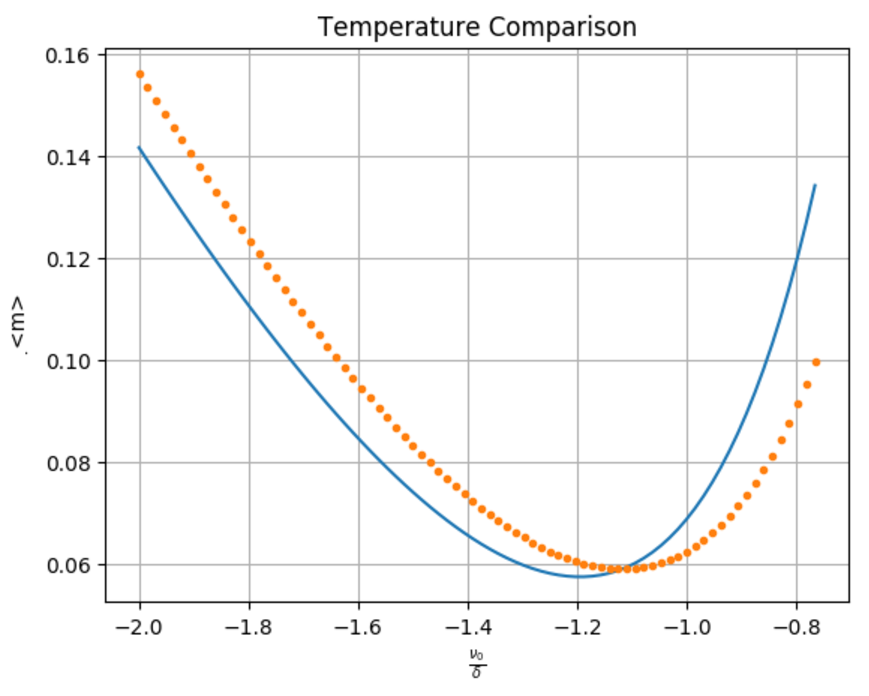
\includegraphics[scale=.55]{GraficaTemp.pdf} 
\caption{\textit{Comparación entre predicciones con y sin el término $\epsilon$} La línea puntuada representa la predicción sin dependencia temporal y la línea sólida representa la predicción con el término adicional. Esta resulta en un mínimo más pequeño de excitaciones posibles y en un corrimiento en el punto donde se espera encontrar este mínimo. Se utiliza $\kappa \ll \nu_0$}
\end{figure}

\fxnote{Falta discutir la figura en el texto}

\chapter{Enfriamiento Optomecánico Dependiente del Tiempo: Caso de Cavidad con Frecuencia Dependiente del Tiempo}

Como se puede observar en el capítulo anterior, el cambio en el comportamiento predicho por el modelo con dependencia temporal es notorio. Sin embargo, durante todas las derivaciones se asume que la cavidad tiene un solo modo de frecuencia constante $\omega_c$. La frecuencia de resonancia de una cavidad de Fabry-Perot, asumiendo que su interior se encuentre en el vacío, está dada por

\begin{equation}
\omega_c = \frac{nc}{2L},
\end{equation} donde $c$ es la velocidad de la luz en el vacío, $n$ es algún entero y $L$ es la longitud de la cavidad. Al emplear un montaje optomecánico como el que se lleva a los resultados del capítulo anterior, $L$ deja de ser constante. Si el oscilador mecánico tiene oscilaciones de amplitud $A$ y se toma a $L_0$ como la longitud promedio de la cavidad, la longitud de la cavidad como función del tiempo viene dada por

\begin{equation}
l(t) = l_0 - A cos(2\omega t)
\end{equation} lo cual lleva a la frecuencia 

\begin{align}
\nu(t) =& \frac{nc}{2l_0-2Acos(2\omega t)}, \\
\approx& \frac{nc}{2l_0} + \frac{nc Acos(2\omega t)}{4l_0^2}, \\
=& \frac{nc}{2l_0} + \frac{nc}{2l_0}(\frac{A}{l_0})cos(2\omega t), \\
=& \omega_0 + \epsilon\omega_0 cos(2\omega t), \\
=& \omega_0(1+\epsilon\ cos(2\omega t)).
\end{align} donde la expresión se deja en primer orden del parámetro de perturbación $\epsilon = \frac{A}{l_0}$. Bajo estas restricciones se tiene un sistema de oscilador armónico donde la frecuencia natural es una función periódica del tiempo. Esto permite el uso de los operadores de Floquet vistos en el capítulo anterior. Se busca un Hamiltoniano optomecánico expresado en términos de estos operadores. Para este fin se hace referencia a la derivación del Hamiltoniano optomecánico general en \cite{LawOH}. Reduciendo la expresión a un solo modo para la cavidad, se tiene la expresión

\begin{equation}
H = \frac{1}{2m}(p + \frac{g}{q} PQ)^2 + v(q) + \frac{1}{2}[P^2+\nu^2 (t)Q^2].
\end{equation} Los operadores $p$ y $q$ corresponden al oscilador mecánico y $P$ y $Q$ al campo dentro de la cavidad. $g$ es una constante. En el trabajo original la dependencia de la frecuencia es sobre la variable $q$ y no precisamente $t$. El teorema de Floquet permite obtener las soluciones de la ecuación

\begin{equation}
\ddot{q} + \nu^2(t)q=0,
\end{equation} y se les llama $f(t)$ y $f(t)^*$. De acuerdo con \cite{HanngiFM} los operadores de Floquet se pueden expresar como

\begin{equation}
\Gamma(t) = \frac{1}{2i}(Q\sqrt{\frac{2m}{\hbar}}\dot{f}(t)-P\sqrt{\frac{2}{m\hbar}}f(t))
\end{equation} y

\begin{equation}
\Gamma(t)^\dagger = \frac{-1}{2i}(Q\sqrt{\frac{2m}{\hbar}}\dot{f}^*(t)-P\sqrt{\frac{2}{m\hbar}}f^*(t)).
\end{equation} A futuro se omite la dependencia temporal de los operadores $\Gamma$ al darse por entendida. Se puede invertir el sistema de ecuaciones y obtener

\begin{align}
Q =& \frac{b^* \Gamma - b \Gamma^\dagger}{(b^* a - a^*b)},\\
P =& \frac{a^* \Gamma - a \Gamma^\dagger}{(b^* a - a^*b)}.
\end{align} donde

\begin{align}
a =& \frac{1}{2i}\sqrt{\frac{2m}{\hbar}} \dot{f}(t),\\
b =& \frac{1}{2i}\sqrt{\frac{2}{m\hbar}} f(t).
\end{align} Esto se sustituye en el término $PQ$ del Hamiltoniano y se obtiene

\begin{equation}
H = \frac{1}{2m}(p + \frac{g}{q} \gamma)^2 + v(q) + \frac{1}{2}[P^2+\nu^2 (t)Q^2],
\end{equation} donde

\begin{equation}
\gamma = \frac{\hbar^2}{W^2 q}[ab^*\Gamma^\dagger \Gamma + a^*b \Gamma \Gamma^\dagger - a^*b^* \Gamma \Gamma - ab \Gamma^\dagger \Gamma^\dagger]
\end{equation} con

\begin{equation}
W= \frac{\dot{f}(t)f^*(t)-\dot{f}^*(t)f(t)}{2i}.
\end{equation}
Esto contrasta con la aproximación realizada en el trabajo original
donde los operadores de creación y aniquilación de la cavidad se
expanden en una serie de potencias para aproximar la dependencia de
estos sobre el operador $q$ del oscilador mecánico. En este
procedimiento se asume $q = l_o + x_m$. En este trabajo asumimos
$x_m = -Acos(\omega t)$. Tomamos al término $\gamma$ en el punto
$q=l_0$

\fxnote{Creo que esta mal la forma en la que hiciste el cálculo. Te
  debo una disculpa por tardarme tanto en darme cuenta. En el artículo
  de CK Law ya supone que la frecuencia depende de la posición, como
  la posición depende del tiempo, el cálculo de CK Law incluye que la
  frecuencia depende del tiempo, por lo tanto no es consistente
  ponerle otra dependencia temporal como lo haces. Sin embargo tu idea
  me parece muy buena si lo que haces es expandir la solución del
  problema clásico en soluciones de Floquet en lugar de lo que hace CK
  Law. Creo que debemos explorar ese camino ahora que defiendas tu
  candidatura. Hablamos mas skype en estos dias. Creo que este
  capítulo lo tienes que reescribir simplemente poniendo la ecuacion
  estandar de CK Law con la disipación de Hangi y decir que
  intentarmos resolverlo. Agregar tambien que exploraremos la
  alternativa que te dije al principio de este comentario.}


Para lidiar con el primer término del Hamiltoniano se emplea la transformación unitaria dada por el operador

\begin{equation}
T = e^\frac{i x_m \gamma}{\hbar}.
\end{equation} Bajo esta transformación 

\begin{align*}
T^\dagger p T =& p - \gamma, \\
T^\dagger p^2 T =& p^2 -2p\gamma, \\
T^\dagger \gamma T =& \gamma,
\end{align*} por lo que, despreciando el término $\gamma^2$ por ser del orden de $\frac{1}{l_0^2}$

\begin{equation}
\frac{1}{2m}(p + \frac{g}{q} \gamma)^2 \approx \frac{p^2}{2m}.
\end{equation} Se conoce como, bajo los operadores de Floquet, los operadores $P$ y $Q$ corresponden a un Hamiltoniano con la forma funcional de un oscilador armónico cuántico usual. Por esto, queda aplicar la transformación al término $\Gamma^\dagger \Gamma$. Cortando a primer orden en $\epsilon$

\begin{align*}
e^{\frac{-ix\gamma_0}{\hbar}}\Gamma^\dagger \Gamma e^{\frac{ix\gamma_0}{\hbar}} =& \Gamma^\dagger \Gamma + [\Gamma^\dagger \Gamma, \gamma_0], \\
=& \Gamma^\dagger \Gamma + \frac{2i\hbar x}{W^2 l_0}(a^*b \Gamma^\dagger \Gamma + a^*b^* \Gamma \Gamma -ab\Gamma^\dagger \Gamma^\dagger),\\
\approx & \Gamma^\dagger \Gamma + \frac{2i\hbar x}{W^2 l_0} a^*b \Gamma^\dagger \Gamma, \\
=& \Gamma^\dagger \Gamma - \frac{i \dot{f}^*(t)f(t) }{W^2 l_0} x  \Gamma^\dagger \Gamma,
\end{align*} de esta forma la constante de proporcionalidad de la presión de radiación es una cantidad dependiente del tiempo bajo este enfoque. Esto contrasta con la definición usual $F= \frac{\omega_0 \hbar}{l_0}$. Tomando en cuenta el factor de amplitud global para el Hamiltoniano de oscilador armónico con frecuencia natural dependiente del tiempo $\frac{W}{|f(t)|^2}$ se obtiene

\begin{equation}
H_{cav} = \frac{\hbar W}{|f(t)|^2}\Gamma^\dagger \Gamma - \frac{\hbar i\dot{f}^*(t)f(t) }{|f(t)|^2W l_0}x  \Gamma^ \dagger \Gamma,
\end{equation} lo cual lleva a identificar el nuevo coeficiente de fuerza $F$ el cual es ahora una función del tiempo

\begin{equation}
F(t) = \frac{\hbar i\dot{f}^*(t)f(t) }{|f(t)|^2W l_0},
\end{equation} y a un Hamiltoniano para un oscilador optomecánico de la forma

\begin{equation}
H = \hbar \omega b^\dagger b + \hbar\frac{ W}{|f(t)|^2}\Gamma^\dagger \Gamma -F(t)x\Gamma^\dagger \Gamma,
\end{equation} pero $x$ es el operador de posición del espejo, el cual se puede expresar en términos de los operadores de creación y aniquilación del oscilador armónico mecánico

\begin{equation}
H = \hbar \omega b^\dagger b + \hbar\frac{ W}{|f(t)|^2}\Gamma^\dagger \Gamma -g(t)\Gamma^\dagger \Gamma(b^\dagger + b),
\end{equation} donde $g$ es una función del tiempo que modula la fuerza de la interacción y está dada por

\begin{equation}
g(t) = \sqrt{\frac{\hbar}{2m\omega}}F(t).
\end{equation}

A este Hamiltoniano se le agrega un término correspondiente a una bomba láser

\begin{equation}
H_{bomba}= \hbar \frac{\Omega}{2}(\Gamma^\dagger + \Gamma).
\end{equation} Y lleva a un Hamiltoniano completo

\begin{equation}
H = \hbar \omega b^\dagger b + \hbar\frac{ W}{|f(t)|^2}\Gamma^\dagger \Gamma -g(t)\Gamma^\dagger \Gamma(b^\dagger + b) + \hbar \frac{\Omega}{2}(\Gamma^\dagger + \Gamma).
\end{equation}

 La ecuación maestra que corresponde a este Hamiltoniano toma en cuenta los intercambios de energía del sistema con el ambiente, tanto la pérdida de fotones de la cavidad como la re-termalización del oscilador mecánico. Esta es \cite{BarberisLC}

\begin{equation} \label{LCMasterEquation}
\dot{\rho} = \frac{1}{i\hbar}[H,\rho] +L_b\rho + L_\Gamma \rho
\end{equation}

Los términos $L$ representan los intercambios de energía con el ambiente. Corresponden al oscilador mecánico y a la cavidad respectivamente. De forma explícita

\begin{align}
L_b \rho =& - \frac{\gamma}{2}(n_m + 1)[b^\dagger b\rho + \rho b^\dagger b -2b\rho b^\dagger]  \\
 &- \frac{\gamma}{2}(n_m)[ bb^\dagger\rho + \rho  bb^\dagger -2b^\dagger\rho b].\nonumber
\end{align} 

\begin{align}
L_\Gamma \rho =& - \frac{\kappa}{2}(n_c + 1)[\Gamma^\dagger \Gamma\rho + \rho \Gamma^\dagger \Gamma -2\Gamma\rho \Gamma^\dagger]  \\
 &- \frac{\kappa}{2}(n_c)[ \Gamma\Gamma^\dagger\rho + \rho  \Gamma\Gamma^\dagger -2\Gamma^\dagger\rho \Gamma].\nonumber
\end{align}

$n_m$ y $n_c$ representan el número promedio de excitaciones térmicas y $\gamma$ y $\kappa$ modelan la pérdida de energía ante el ambiente. Para poder estudiar este sistema se hace una transformación a  un marco de referencia desplazado, esto se estudia en detalle en el próximo capítulo.

\chapter{Transformación al Marco de Referencia Desplazado}

Esta transformación se utiliza para eliminar términos de orden tercero en operadores en la ecuación \eqref{LCMasterEquation}. La transformación es unitaria y se genera mediante el operador

\begin{equation}
U_{b,\Gamma} =  U_b U_\Gamma = e^{(\beta b^\dagger - \beta^* b)}e^{(\alpha\Gamma^\dagger - \alpha^* \Gamma)}.
\end{equation} $\alpha$ y $\beta$ son coeficientes complejos dependientes del tiempo que se elijen de manera conveniente para simplificar la ecuación maestra. Se busca una ecuación para la matriz densidad no transformada \cite{TesisMaestria}. Bajo la transformación la matriz densidad es

\begin{equation}
\rho' = U_{b,\Gamma}^\dagger \rho U_{b,\Gamma}.
\end{equation} Se puede despejar en términos de $\rho$, utilizando el hecho de que la transformación es unitaria

\begin{equation}
\rho = U_{b,\Gamma} \rho' U_{b,\Gamma}^\dagger,
\end{equation}y derivando respecto al tiempo

\begin{equation}
\dot{\rho} = L\rho = \frac{d}{dt}(U_{b,\Gamma} \rho' U_{b,\Gamma}^\dagger).
\end{equation} En este caso, $L$ representa el operador de Liouville. Esto permite obtener una ecuación maestra para $\rho'$. 

\begin{align}
 U_{b,\Gamma} \dot{(\rho')} U_{b,\Gamma}^\dagger =& L[U_{b,\Gamma} \rho' U_{b,\Gamma}^\dagger] - \dot{U}_{b,\Gamma}\rho'U_{b,\Gamma}^\dagger -U_{b,\Gamma} \rho' \dot{U}_{b,\Gamma}^\dagger\\
\dot{\rho} =& U_{b,\Gamma}^\dagger L[U_{b,\Gamma} \rho' U_{b,\Gamma}^\dagger]U_{b,\Gamma}-U_{b,\Gamma}^\dagger\dot{U}_{b,\Gamma}\rho'-\rho'\dot{U}_{b,\Gamma}^\dagger U_{b,\Gamma}.
\end{align} A partir de este punto, se omiten los sub-índices de las transformaciones y la $'$ para la matriz densidad. La transformación afecta a los distintos operadores presentes en el Hamiltoniano de la siguiente forma

\begin{align}
U^\dagger b U =& b + \beta,\\
U^\dagger \Gamma U =& \Gamma + \alpha,\\
U^\dagger b^\dagger b U =& b^\dagger b + \alpha^* b + \alpha b^\dagger +|\beta|^2,\\
U^\dagger \Gamma^\dagger \Gamma U =& \Gamma^\dagger \Gamma + \alpha^* \Gamma + \alpha \Gamma^\dagger +|\alpha|^2.
\end{align} Los conjugados Hermitianos se obtienen de manera trivial. Utilizar operadores con dependencia temporal explícita añade complejidad adicional a este procedimiento debido a las derivadas temporales del operador $U$. El procedimiento completo puede encontrarse en \cite{TesisMaestria}. Se obtiene

\begin{align}
\dot{U}_b=&\dot{\beta} b^\dagger U_b - U_b\dot{\beta}^*b - \frac{1}{2}(\dot{\beta} \beta^*+\dot{\beta}^* \beta)U_b,\\
\dot{U}_b^\dagger=&-\dot{\beta} b^\dagger U_b^\dagger + U_b^\dagger\dot{\beta}^*b - \frac{1}{2}(\dot{\beta} \beta^*+\dot{\beta}^* \beta)U_b^\dagger.
\end{align} El caso de $U_\Gamma$ es más complejo, pero el procedimiento es equivalente. Se obtiene

\begin{align}
\dot{U}_\Gamma =&(\dot{\alpha}\Gamma^\dagger +\alpha \dot{\Gamma}^\dagger)U_\Gamma - U_\Gamma(\dot{\alpha}^*\Gamma+\alpha^* \dot{\Gamma}) + (\alpha^*)^2 C_{--}(t)U_\Gamma-\frac{1}{2}(\dot{\alpha} \alpha^*+\dot{\alpha}^* \alpha)U_\Gamma, \\
\dot{U}^\dagger_\Gamma=&-(\dot{\alpha}\Gamma^\dagger +\alpha \dot{\Gamma}^\dagger)U_\Gamma^\dagger + U_\Gamma^\dagger(\dot{\alpha}^*\Gamma+\alpha^* \dot{\Gamma}) - (\alpha)^2 C_{++}(t)U_\Gamma^\dagger-\frac{1}{2}(\dot{\alpha} \alpha^*+\dot{\alpha}^* \alpha)U_\Gamma^\dagger.
\end{align} Finalmente se debe calcular las transformaciones de las derivadas temporales de los operadores $\Gamma$

\begin{align}
U^{\dagger}\dot{\Gamma}U =& \dot{\Gamma} + \alpha C_{-+}(t) -\alpha^* C_{--}(t),\\
U^{\dagger}\dot{\Gamma}^\dagger U =& \dot{\Gamma}^\dagger - \alpha^* C_{+-}(t) +\alpha C_{++}(t). 
\end{align} Los coeficientes $C(t)$ surgen debido a que los operadores $\Gamma$ no necesariamente conmutan con sus derivadas temporales

\begin{align*}
C_{++}(t) =& [\dot{\Gamma}^{\dagger}, \Gamma^{\dagger}],\\
C_{+-}(t) =& [\dot{\Gamma}^{\dagger}, \Gamma],\\
C_{-+}(t) =& [\dot{\Gamma}, \Gamma^{\dagger}],\\
C_{--}(t) =& [\dot{\Gamma}, \Gamma].
\end{align*} Falta únicamente calcular los términos de la ecuación maestra que corresponden a estas derivadas temporales

\begin{equation}
U_b^\dagger \dot{U}_b \rho + U_\Gamma^\dagger \dot{U}_\Gamma \rho + \rho \dot{U}_b^\dagger U_b+ \rho \dot{U}_\Gamma^\dagger U_\Gamma,
\end{equation} los cuales resultan ser

\begin{align}
U_\Gamma^\dagger \dot{U}_\Gamma \rho &= [(\dot{\alpha}\Gamma^\dagger + \alpha \dot{\Gamma}^\dagger - \dot{\alpha}^*\Gamma -\alpha^*\dot{\Gamma} ) \\
 &- |\alpha|^2C_{+-} + (\alpha)^2C_{++} + (\alpha^*)^2 C_{--} - \frac{1}{2}\dot{|\alpha^2|} + \dot{\alpha}^*\alpha]\rho \nonumber,
\end{align}

\begin{align}
 \rho \dot{U}_\Gamma^\dagger U_\Gamma &= \rho[(-\dot{\alpha}\Gamma^\dagger - \alpha \dot{\Gamma}^\dagger + \dot{\alpha}^*\Gamma +\alpha^*\dot{\Gamma} ) \\
 &+ |\alpha|^2C_{-+} - (\alpha)^2C_{++} - (\alpha^*)^2 C_{--} - \frac{1}{2}\dot{|\alpha^2|} + \dot{\alpha}\alpha^*], \nonumber
\end{align}

\begin{align}
U_\Gamma^\dagger \dot{U}_\Gamma \rho + \rho \dot{U}_\Gamma^\dagger U_\Gamma &= [\rho, (\alpha^*\dot{\Gamma} - \alpha\dot{\Gamma}^\dagger)] + [\rho, (\dot{\alpha}^*\Gamma - \dot{\alpha}\Gamma^\dagger)] \\
&+|\alpha|^2 (C_{-+} - C_{+-}).
\end{align} 

Los términos que involucran un conmutador con la matriz densidad se consideran parte del Hamiltoniano. El procedimiento para los términos  $U_b$ es el mismo pero resulta más sencillo

\begin{equation}
U_b^\dagger \dot{U}_b \rho+ \rho \dot{U}_b^\dagger U_b = [\rho, (\dot{\beta}^*b - \dot{\beta}b^\dagger)].
\end{equation} El Hamiltoniano queda entonces dado por

\begin{align}
H_{mec}' =& \hbar \omega(b^{\dagger}b +\beta b^{\dagger}+\beta^* b + |\beta|^2),\\
H_{cav}' =& \hbar\frac{W}{|f(t)|^2}(\Gamma^{\dagger}\Gamma + \alpha \Gamma^{\dagger} + \alpha^* \Gamma + |\alpha|^2 ),\\
H_{rad}'=&-\hbar g(t)[(\Gamma^{\dagger}\Gamma + \alpha \Gamma^{\dagger} + \alpha^* \Gamma + |\alpha|^2 )((b^{\dagger}+\beta^*)+(b+\beta))],\\
B' =& \frac{\hbar \Omega}{2}(\Gamma^{\dagger} + \Gamma +\alpha + \alpha^*).
\end{align}

Más términos adicionales generados por la transformación debido a sus derivadas temporales

\begin{equation}
H_{T} = (\alpha^*\dot{\Gamma} - \alpha\dot{\Gamma}^\dagger) +(\dot{\alpha}^*\Gamma - \dot{\alpha}\Gamma^\dagger) +(\dot{\beta}^*b - \dot{\beta}b^\dagger),
\end{equation} y debido a los términos de Lindblad

\begin{equation}
U^\dagger [L_aU\rho U^\dagger]U + U^\dagger [L_\Gamma U\rho U^\dagger]U,
\end{equation} se generan términos adicionales para el Hamitloniano mientras que los términos de Lindblad mantienen su forma original

\begin{align}
U^\dagger [L_bU\rho U^\dagger]U=& L_b\rho + [\beta b^\dagger - \beta^* b,\rho],\\
U^\dagger [L_\Gamma U\rho U^\dagger]U =& L_\Gamma \rho + [ \alpha \Gamma^\dagger - \alpha^* \Gamma,\rho].
\end{align} La transformación de los términos Lindblad resulta en  Hamiltoniano efectivo adicional

\begin{equation}
H_L = -\frac{\gamma}{2}(\beta b^\dagger + \beta^* b) -\frac{\kappa}{2}( \alpha \Gamma^\dagger + \alpha^* \Gamma).
\end{equation} A fin de simplificar el Hamiltoniano, es necesario agrupar todos los términos a primer orden en operadores

\begin{align}
&b(\omega\beta - g(t)|\alpha|^2 + i\dot{\beta}^* + i\frac{\gamma}{2}\beta),\\
&\Gamma(\frac{W\alpha}{|f|^2} -g(t)\alpha(\beta^*+\beta) + \frac{\Omega}{2}-i\dot{\alpha} - i\frac{\kappa}{2}\alpha),
\end{align} y sus conjugados Hermitianos. Para anular estos términos es necesario que se cumpla el sistema de ecuaciones diferenciales

\begin{align}
&\dot{\beta} = -i\omega\beta^* + ig(t)|\alpha|^2 - \frac{\gamma}{2}\beta,\\
&\dot{\alpha} = -i \frac{W}{|f|^2}\alpha^* + ig(t)\alpha(\beta + \beta^*) -i \frac{\Omega}{2} - \frac{\kappa}{2}\alpha^*.
\end{align} Debido a la forma de la frecuencia elegida, la función $f(t)$ que figura en los operadores $\Gamma$ es

\begin{equation}
f(t) = e^{i\omega t} + \frac{\epsilon}{16}e^{3i\omega t}
\end{equation} por lo que si se desprecian términos de corrección menores a epsilon

\begin{align}
\dot{\Gamma}(t) =& i\omega \Gamma(t),\\
\dot{\Gamma}^\dagger(t) =& -i\omega \Gamma^\dagger(t),
\end{align} y estos términos deben incluirse en las ecuaciones para $\alpha$ y $\beta$

\begin{align}
&\dot{\beta} = -i\omega\beta^* + ig(t)|\alpha|^2 - \frac{\gamma}{2}\beta,\\
&\dot{\alpha} = -i \frac{W}{|f|^2}\alpha^* + ig(t)\alpha(\beta + \beta^*) -i \frac{\Omega}{2} - \frac{\kappa}{2}\alpha^* + \omega\alpha^*.
\end{align} El caso de interés es el caso estacionario $\dot{\alpha}=\dot{\beta} = 0$. Se trabaja el límite de acoplamiento pequeño y se limita el análisis a orden 0 en el parámetro de acoplamiento $g(t)$

\begin{align}
&0 = -i\omega\beta^* - \frac{\gamma}{2}\beta,\\
&0 = -i \frac{W}{|f|^2}\alpha^* -i \frac{\Omega}{2} - \frac{\kappa}{2}\alpha^* + \omega\alpha^*.
\end{align} dada la expresión para $f(t)$ se tiene

\begin{equation}
\frac{W}{|f(t)|^2} = \omega,
\end{equation} se llega a la solución, a orden 0 en acoplamiento

\begin{align}
\beta_0 =& 0, \\
\alpha_0 =& \frac{\Omega}{-i\kappa - 2\omega(1-i)}.
\end{align} lo cual resulta en el Hamiltoniano transformado

\begin{equation}
H = \hbar \omega b^\dagger b + \hbar\omega \Gamma^\dagger \Gamma -\hbar g(t)[( \alpha \Gamma^{\dagger} + \alpha^* \Gamma)(b^{\dagger}+b)]
\end{equation} donde se ha despreciado el término $\Gamma^{\dagger}\Gamma$ en la interacción ya que en este régimen $|\alpha| \gg 1$ y es despreciable respecto a los otros dos términos. De esta forma se tiene un nuevo Hamiltoniano para interacción optomecánica donde se modela que la intensidad de la interacción optomecánica es una función del tiempo.

\chapter{Objetivos Futuros}


A partir del Hamiltoniano obtenido es posible estudiar un sistema de gran importancia tomando en cuenta su dependencia temporal inherente, la cual se no se mantiene en el Hamiltoniano usual\cite{CavesIF}. A partir de este punto se proponen tres objetivos para realizar un estudio más completo de este sistema bajo este nuevo enfoque. En todos los casos se espera obtener expresiones analíticas y resultados numéricos  para la temperatura final del oscilador mecánico bajo la aproximación adiabática.

\section{Objetivos y Calendarización}

\begin{enumerate}
\item Llegar a una expresión para la temperatura final del espejo bajo la aproximación adiabática y compararla con la expresión usual que se obtiene al no considerar una dependencia temporal explícita para la frecuencia natural de la cavidad. Esto requiere deducir desde primeros principios la ecuación maestra que contiene los coeficientes de enfriamiento y calentamiento correspondientes al oscilador mecánico.

\item Estudiar el sistema en un régimen distinto al establecido en los capítulos anteriores. Si no se puede tomar la interacción a orden cero durante la transformación al marco desplazado esto cambia el coeficiente $\alpha$ y lo convierte en una función del tiempo.

\item Estudiar el sistema cuando el parámetro $\epsilon$ debe tomarse en cuenta hasta segundo orden. Este cambio lleva a que incluso el factor global del Hamiltoniano para el campo dentro de la cavidad sea una función del tiempo, lo que lleva a estudiar el efecto sobre el oscilador de interactuar con un campo cuya frecuencia natural oscila en el tiempo. 
\end{enumerate}

Se prevee que cada uno de estos objetivos, junto con trabajo de redacción y revisión bibliográfica adicional, sea realizable dentro de un semestre de trabajo. Esto implicaría un último semestre únicamente dedicado a redacción a fin de elaborar la tesis doctoral en tiempo y forma, así como un artículo de investigación a ser publicado en una revista internacional.









\bibliographystyle{unsrt}
\bibliography{Bib}

\end{document}
